%------------------------------------------------------------------------------------------------
\section{Regulationsmöglichkeiten}
\label{sec:Regulationsmöglichkeiten}
%------------------------------------------------------------------------------------------------

Neben bereits entwickelten Werkzeugen für das Vermeiden der Erhebung personenbezogener Daten existieren gleicherweise unzählige theoretische Konzepte, die unter Verwendung verschiedenster Herangehensweisen die Datenerhebung entweder regulieren oder ganz unterdrücken. 
Zu beachten ist, dass aufgrund der in \fullref{sec:Grundlagen} vorgestellten Architektur einer \ac{iot}-Anwendung beziehungsweise eines Systems, unterschiedliche Ansätze zur Verfügung stehen, um als Entwickler oder Nutzer Einfluss auf das Verhalten eines Gerätes zu nehmen. 
Nachfolgend wird nun beginnend mit einer allgemeinen Einführung in die Grundlagen der Regulierung, eine Reihe von Konzepten und Technologien vorgestellt, die innerhalb dieses Kontextes Verwendung finden, und somit als State-of-the-Art Ansätze deklariert werden können. Hierbei ist jedoch zu beachten, dass aufgrund der meist nur theoretischen Methoden nicht von finalen und in der breiten Masse eingesetzten Verfahren gesprochen werden kann. 
Schließlich werden auf Basis der angefertigten Bewertungen noch zwei Beispiele aufgezeigt, die es erlauben eine Datenschutzkonformität in Bezug auf die \ac{dsgvo} herzustellen.

%------------------------------------------------------------------------------------------------
\subsection{Grundlagen der Regulierung}
\label{sec:Regulationsmöglichkeiten:ssec:Grundlagen der Regulierung}
%------------------------------------------------------------------------------------------------

Entsprechend der Abbildung \ref{fig:drei-schichten-iot}, kann eine \ac{iot}-Applikation beziehungsweise Architektur in unterschiedliche Schichten (\textbf{\textit{Layer}}) eingeteilt werden. Neben einem \textbf{Application Layer}, kann in einen \textbf{Perception} und einen \textbf{Sensing Layer} unterschieden werden. 
Auf Basis dieses Schichtenkonstruktes setzen die einzelnen Werkzeuge jeweils an einer Schicht oder Schichtenübergreifend zur Umsetzung ihrer implementierten Regulationen an. Die als am häufigsten verwendete Schnittstelle zur Implementierung konnte, im Bezug auf die betrachtete Literatur, als der \textbf{Perception Layer} identifiziert werden, in dem sich beispielsweise das Netzwerk befindet. 
Hier wird direkt auf Paketebene der Kontakt zu ungewollten Kommunikationspartnern oder die Observierung von unverschlüsselten Netzwerkverkehr mit sensiblen Informationen möglich und kann nach Wunsch unterbunden werden. Andererseits besteht die Möglichkeit auch auf dem \textbf{Application Layer} anzusetzen, womit größtenteils die Umsetzung von Sicherheitsrichtlinien im Bezug auf \ac{sbd} und \ac{pbd} beschrieben werden. 
Konzeptionelle Ansätze wie die in der nachfolgenden Sektion \fullref{sec:Regulationsmöglichkeiten:ssec:State-of-the-Art} beschriebenen ''Snap4City'' Architektur \cite{Badii2020} schließen im Regelfall mehrere Schichten mit ein. 
Dies ist überwiegend auf die vollumfängliche Betrachtung der gesamten Systemlandschaft zurückzuführen, die neben den betriebenen Anwendungen, auch deren Kommunikation (Netzwerk) und den Aufbau der Geräte selbst definiert.

%------------------------------------------------------------------------------------------------
\subsection{State-of-the-Art}
\label{sec:Regulationsmöglichkeiten:ssec:State-of-the-Art}
%------------------------------------------------------------------------------------------------

Anwendung von Ansätzen, die für die Umsetzung von mehr Sicherheit und Privatsphäre verwendet werden können, gibt es bereits in dieser Form innerhalb anderer Systeme. 
Häufig werden beispielsweise Methoden wie Authentifizierung und Zugriffskontrolle in Verbindung mit verschlüsseltem Datenverkehr als Sicherheitsmaßnahmen aufgeführt, um unbefugten Zugriff auf die gespeicherten Daten zu präventieren \cite{SecPrivSmartCity2021}. 
Im Kontext der Smart City ist eine exemplarische Umsetzung in Form der ''Snap4City'' Architektur \cite{Badii2020} erfolgt, die basierend auf unterschiedlichen Plattformen, auf denen die einzelnen Dienste lokalisiert sind, über OpenID Connect und OAuth2 die Authentifizierung und Autorisierung postuliert. 
Hierbei lassen sich neben rein token-basierten Verfahren für die Identifikation von menschlichen Nutzern, auch Zertifikate für die Integration auf Geräteebene einsetzen. 
Dies ermöglicht neben der gezielten Differenzierung zwischen einzelnen Nutzern auch eine Identifikation einzelner Geräte basierend auf ihren Zertifikaten. 
Weitere Ansätze, die derzeit innerhalb unterschiedlichster Arbeiten diskutiert werden, sind mitunter Konzepte, die neben den bereits genannten Sicherheitsvorkehrungen zusätzlich auf die Verwendung von neuesten Technologien wie zum Beispiel Blockchain, Machine Learning oder Ontologie-basierten Verfahren aufsetzen \cite{Cui2018}. 
Da es sich hierbei aber nur um theoretische Entwürfe handelt, die bisher noch in keinen praxistauglichen Implementierung angewendet wurden, werden hier nur die zugrundeliegenden Technologien genannt. 
Auch im Rahmen von Quantum Computing sind bereits Konzepte für den Einsatz innerhalb von Smart City Lösungen in Entwicklung \cite{Bashirpour2022}. 

%------------------------------------------------------------------------------------------------
\subsection{IoTrimmer \& IoTrigger}
\label{sec:Regulationsmöglichkeiten:ssec:IoTrimmer und IoTrigger}
% Network Layer
%------------------------------------------------------------------------------------------------

Beginnend mit dem ersten Werkzeug, welches aus der Arbeit \cite{Mandalari2021} zur Identifikation von nicht für die Dienstbereitstellung benötigten Datenverkehrs eingesetzt werden konnte. Bei genauerer Betrachtung handelt es sich bei IoTrimmer und IoTrigger \cite{Mandalari2021} um zwei Skripte, die platziert auf einem Router, der die Schnittstelle für die jeweiligen Geräte darstellt, den generierten Datenverkehr analysieren. 
Maßgeblich für die Nutzung ist somit ein abgeschlossenes Netzwerk, dass die zu regulierenden Geräte enthält. Dies bedeutet im Umkehrschluss, dass es sich hierbei um ein Tool für die Verwendung im \textbf{Smart Home} Umfeld handelt und bezüglich des Ansatzpunktes für die Regulation innerhalb des \textbf{Perception Layer} einzuordnen ist.
Die Interaktion der beiden Komponenten lässt sich anhand der nachfolgenden Abbildung \ref{fig:iotrigger-iotrimmer} anschaulich erklären.

\begin{figure}
    \centering
    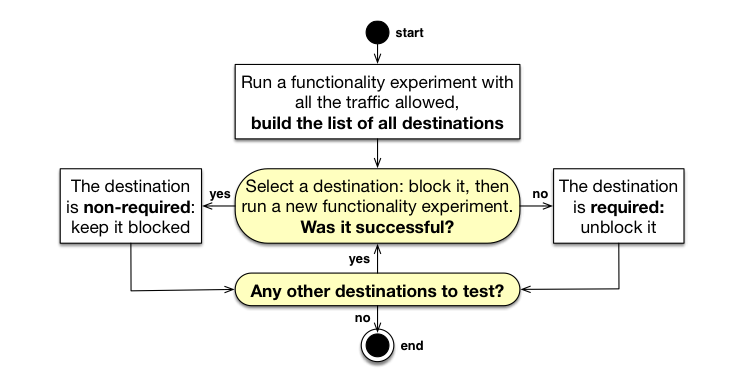
\includegraphics[width=\textwidth]{main/countermeasures/pictures/Identification_Non_Essential_Traffic}
    \caption{Beschreibung des Algorithmus zur Detektion von nicht benötigten Endpunkten, die das Geräte kontaktiert \cite{Mandalari2021}}
    \label{fig:iotrigger-iotrimmer}
\end{figure}

\noindent Im Voraus wird durch den IoTrigger eine Reihe an automatisierten Tests an den zu kontrollierenden Geräten durchgeführt. Hierbei handelt es sich um das Auslösen von gerätespezifische Funktionen, die im Rahmen von \cite[p. 13-14]{Mandalari2021} erstellt wurden und somit nicht universell nutzbar sind. 
Resultierend aus den vorgefertigten Geräte-Tests werden anschließend Listen mit allen angesprochenen Destinationen generiert, die im Zusammenhang einer Interaktion des Nutzers mit dem Gerät entstehen. Daraufhin werden die einzelnen Destinationen iterativ durch den IoTrigger blockiert und die Funktionsfähigkeit des Geräts überprüft. 
Ist das Gerät trotz geblockter Ressource noch voll funktionsfähig, handelt es sich um einen nicht benötigten Endpunkt, der daraufhin weiterhin blockiert bleibt. Andernfalls wird das Ziel als notwendig markiert und für die Verwendung durch das Gerät freigegeben. 
Die abschließend annotierte Liste mit allen notwendigen und nicht notwendigen Endpunkten wird an den IoTrimmer geleitet, der auf Basis der erstellten Auflistung entsprechende Firewall-Regeln erstellt. Dieses Konzept kommt dem Konstrukt von Block- und Allow-Listen gleich, die innerhalb vieler Router umgesetzt sind \cite{FritzBox2022}.
Die Nutzung der Firewall als Regulator für unerwünschten Datenstrom stellt hierbei keine Seltenheit dar. Neben dem hier vorgestellten Werkzeug existieren beispielsweise noch FANE \cite{Haar2019} und SeCoMan \cite{Huertas2016} deren Konzeption auch auf der dynamischen Anpassung der Firewall-Regeln basiert. Grenzen bezüglich dieses Einsatzes sind dennoch, dass keine Regulation auf Basis der gesendeten Daten stattfindet. 
Für die Prüfung von erhobenen Informationen bedingt der Einsatz solch eines Tools, dass der Nutzer selbst den Informationsgehalt der gesendeten Nachrichten prüft und infolgedessen weitere Anpassungen vornimmt. Allerdings handelt es sich um einen ersten Ansatz, um beispielsweise die Verfolgung von gesetzeswidriger Kommunikation mit Diensten außerhalb der Drittländer-Regelung \cite{Dsgvo2016} zu unterbinden.

%------------------------------------------------------------------------------------------------
\subsection{''SmartWalk'' \cite{Natix2022}}
\label{sec:Regulationsmöglichkeiten:ssec:SmartWalk}
% Application Layer
%------------------------------------------------------------------------------------------------

Im Kontrast zu der in der vorherigen Sektion \fullref{sec:Regulationsmöglichkeiten:ssec:IoTrimmer und IoTrigger} beschriebenen Vorgehensweise zur Kontrolle der erhobenen Daten ist die Verwendung einer Lösung auf Netzwerkebene für die Größe eines Ökosystems im Sinne einer \textbf{Smart City} deutlich komplexer umzusetzen. 
Des Weiteren ist es im Gegensatz zu einer kontrollierten Umgebung wie der Behausung eines Smart Home, den Bewohnern einer Stadt größtenteils nicht möglich zu wissen, welche Geräte sich gerade in ihrem Umfeld befinden und welche Daten von den Geräte gesammelt werden. 
Dies setzt die Verwendung anderer Konzepte voraus, die bereits Teil der Anwendungen sind, die auf den einzelnen Geräten betrieben werden. Hierbei kommt in den meisten Fällen \ac{sbd} und \ac{pbd} zum Einsatz, die in Form von theoretischen Paradigmen die Sicherheit beziehungsweise Privatsphäre applikationsseitig umsetzen. 
So auch im Kontext des ''SmartWalk'' \cite{Natix2022} Projektes, welches derzeit in Hamburg umgesetzt wird. Diese Lösung zur Regulation nicht konformer Datenerhebung setzt auf dem \textbf{Application Layer} innerhalb des \ac{iot}-Stacks an.
Wie bereits in \ref{sec:Analyse der Datenerhebung:ssec:Bewertung der Datenschutzkonformität} beschrieben, hat das ''SmartWalk''-Projekt die Zielsetzung das Überqueren von Straßen für Fußgänger und andere Verkehrsteilnehmer unter Verwendung von kameragestützen \ac{iot}-Systemen sicherer zu gestalten. 
Hierzu sammeln die beteiligten Sensoren Bilddaten des laufenden Verkehrs und geben auf Basis von Faktoren wie Geschwindigkeit und Distanz eine Warnung an die Verkehrsteilnehmer auf der Straße ab \cite{SmartWalk2022}. 
Die hierbei erhobenen Daten werden bereits innerhalb des Kamerasystems, auch als Edge-Video-Technologie bezeichnet, durch Prüfung mittels eine KI-Systems entsprechend anonymisiert, sodass am Ende keinerlei Rückschlüsse auf die gefilmten Individuen oder deren Fahrzeuge mehr möglich sind. Ein beispielhafter Ausschnitt aus einer anonymisierten Aufnahme wird in der nachfolgenden Abbildung \ref{fig:anonymized-footage} illustriert.

\begin{figure}
    \centering
    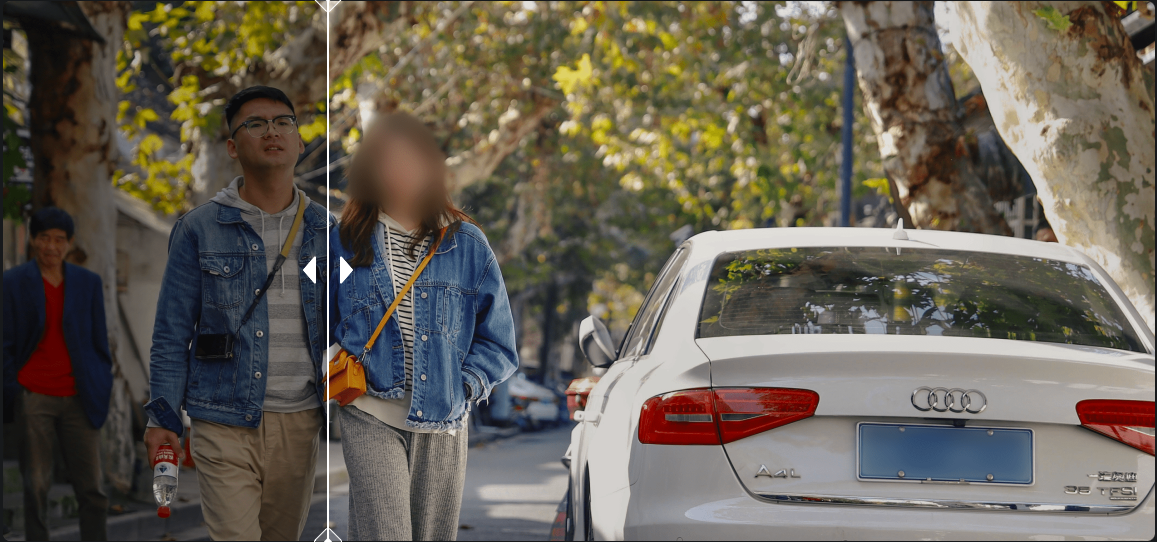
\includegraphics[width=\textwidth]{main/countermeasures/pictures/Anonymized_Footage}
    \caption{Beispiel einer anonymisierten Aufnahme nach der Verarbeitung durch das KI-Modell von NATIX \cite{Natix2022}}
    \label{fig:anonymized-footage}
\end{figure}

Wie auf der Aufnahme zu erkennen ist, wurde das Modell so trainiert, dass es innerhalb einzelner Aufnahmen die Gesichter und Nummernschilder aufgezeichneter Fahrzeuge erkennt und diese gezielt unkenntlich macht. 
Unter Zuhilfenahme von KI-Technologien wäre somit neben der Erkennung von sensiblen Eigenschaften innerhalb ganzer Datensätze auch die Prävention von unzulässiger Verarbeitung der Daten minimiert bis ausgeschlossen, wodurch sich diese Herangehensweise als äußerst effizient für den Einsatz in \textbf{Smart City} Applikationen anbietet.

